\documentclass[10pt]{article}

\usepackage[left=2.5cm,
            right=2cm,
            top=2cm,
            bottom=2cm]{geometry}
\usepackage{hyperref}
\usepackage{fancyhdr}
\usepackage{titling}
\usepackage{verbatim}
\usepackage{amsmath}
\usepackage{graphicx}
\graphicspath{ {./images/} }

\title{DMML - Assignment 2}
\author{Ishita Pethkar (BMC202128), Siddhant Shah (BMC202171)}
\date{$31^{th}$ March, 2024}

\pagestyle{fancy}
\fancyhead{}
\lhead{\href{https: //github.com/SidShah2953/dmml-24-assn-2}{GitHub URL}}
\chead{\thetitle}
\rhead{Ishita Pethkar, Siddhant Shah}

\begin{document}
\thispagestyle{empty}
\maketitle

% \tableofcontents

\section{General Strategy}
\begin{itemize}
    \item \textbf{Representation of Data - Set  Representation:}
    Data is represented as a list of sets where each set represents a document.
        \begin{itemize}
            \item ENRON: Sparsity of $0.331 \%$
            \item KOS: Sparsity of $1.491 \%$
            \item NIPS: Sparsity of $4.006 \%$
        \end{itemize}
        Due to the high sparsity and the efficiency of Python's implementation of sets, we choose to use this representation for the data as we have been asked to disregard the frequency of each word in a document, and rather only focus on its presence or absence.
    \item We evaluate the clustering algorithm for $k = 2$ to $k = 25$. \\
    We start clustering for $k = 2$. The first centroid is chosen at random and the next point is chosen using the method below. 
    \item \textbf{Picking the next centroid - K-Means++ Method:} For $k = k+1$ we retain the initial $k$ centroids and the next centroid is the point having maximum distance from its respective centroid.
    \item The clustering algorithm is run using the Jaccard distance. We stop the clustering if the inertia from the new centroids is higher than that for the old cluster. This is because we vary the threshold depending on the case to make sure that centroids are not empty sets.
    \item We plot the graph of Inertia vs $k$ to find the optimum $k$. The $k$ after which the graph plateaus is the optimum $k$.
\end{itemize}

\section{Results}
    We carry out clustering on Enron, NIPS and KOS dataset using  set representation and K-Means++ method. The optimum value of $k$ is found using the Elbow method.
    \begin{table}[h]
        \begin{center}
            \begin{tabular}{|l|l|l|l|}
                \hline
                Properties &Storage (in bytes) &Time (in minutes) &Optimum $k$\\
                \hline
                ENRON &351064 &1:56 &15 \\
                KOS &29336 &0:15 &12 \\
                NIPS &12728 &0:40 &21 \\
                \hline
            \end{tabular}
        \end{center}
        \caption{Summary of Results}
    \end{table}

    \subsection{ENRON Collection}
        The Enron Emails have $39861$ documents and $28102$ distinct words occurring across them.

        The entire execution takes $1:56$ minutes to execute and reading and storing the data takes 351064 bytes.
        The graph of the $k$ vs Inertia looks as follows, giving us $15$ to be the optimal value for $k$.
        \begin{figure}[h]
            \centering
            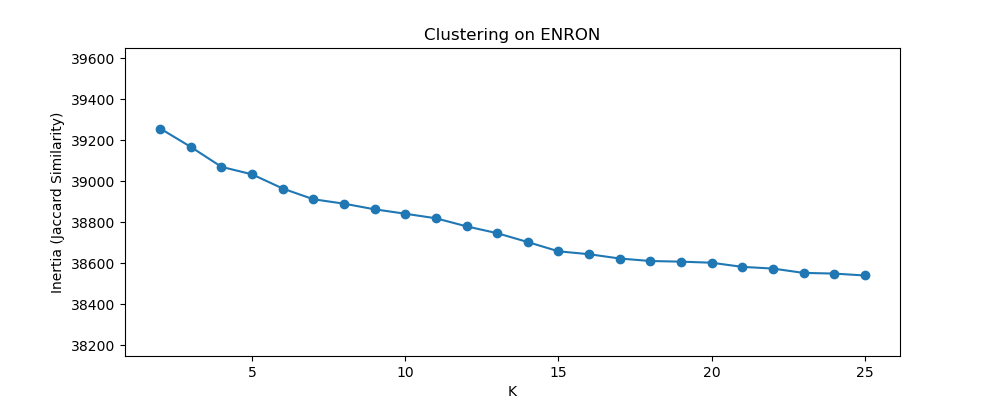
\includegraphics[width=12cm]{ENRON.png}
            \caption{$k$ vs. Inertia for Enron}
            \label{fig:ENRON-Inertia}
        \end{figure}

    \subsection{KOS Collection}
        The Enron Emails have $3430$ documents and $6906$ distinct words occurring across them.

        The entire execution takes $0:15$ minutes to execute and reading and storing the data takes 29336 bytes.The graph of the $k$ vs Inertia looks as follows, giving us $15$ to be the optimal value for $k$.
        \begin{figure}[h]
            \centering
            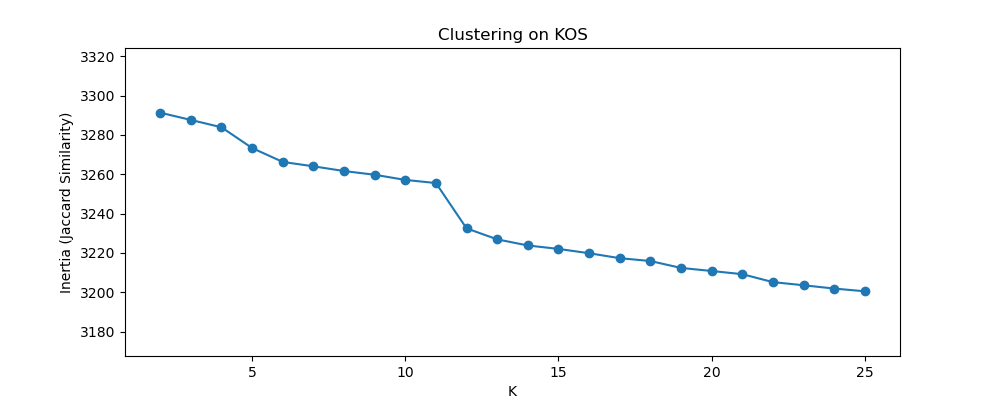
\includegraphics[width=12cm]{KOS.png}
            \caption{$k$ vs. Inertia for KOS}
            \label{fig:KOS-Inertia}
        \end{figure}

    \subsection{NIPS Collection}
        The NIPS Papers have $1500$ documents and $12419$ distinct words occurring across them.

        The entire execution takes $0:40$ minutes to execute and reading and storing the data takes 12728 bytes.
        The graph of the $k$ vs Inertia looks as follows, giving us $21$ to be the optimal value for $k$.
        \begin{figure}[h]
            \centering
            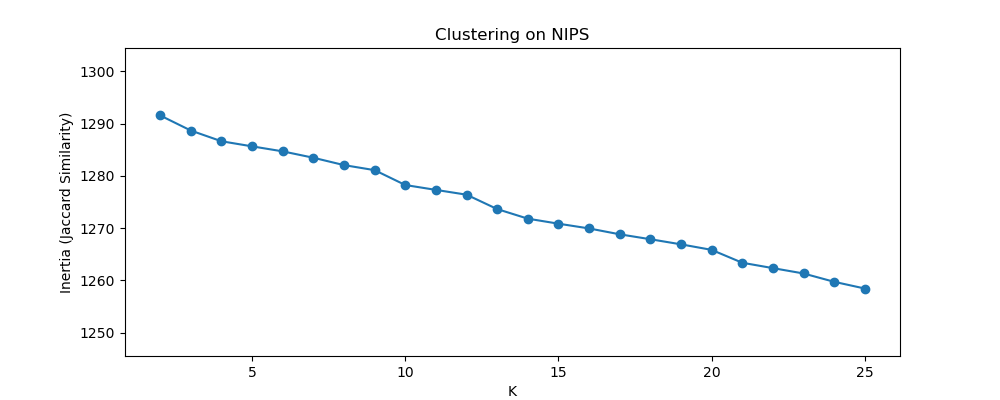
\includegraphics[width=12cm]{NIPS.png}
            \caption{$k$ vs. Inertia for NIPS}
            \label{fig:NIPS-Inertia}
        \end{figure}
\end{document} % End of document body
